\section{Diskussion}
\subsection{Durchgeführte Experimente}
Um die Biomechanik des Gehens zu untersuchen, wurden zwei Versuche durchgeführt: Das stationäre Gehen auf einem Laufband und das Gehen über eine Laufstrecke. Ersteres bietet die Möglichkeit, die Kinematik des Gehens eingehend zu studieren. Stationär deshalb, da die Fortbewegung innerhalb des Raumes gleich null ist. Der Proband kann so seinen Laufrhythmus finden, die Geschwindigkeit kann von außen vorgegeben werden und es können mehrere Schritte hintereinander aufgezeichnet werden. Das Gehen auf der Laufstrecke ermöglicht es, während eines Bodenkontaktes auf der eingebauten Waage die Bodenreaktionskräfte in drei Raumrichtungen aufzunehmen. Gekoppelt mit einer gleichzeitig Laufenden Kamera lassen sich Video- und Kraftmessungen zusammenführen und mit der Methode der inversen Dynamik können die wirkenden Kräfte in den Gelenken des Beines rekonstruiert werden. \\
Bei dem Probanden handelt es sich um einen 24 jährigen Mann, ohne bekannte Gelenkschäden, Haltungsschäden oder anderweite Beeinträchtigungen. 
\textbf{AUSWIRKUNGEN VON SCHUHWERK AUF GEHSTIL?}


\subsection{Bodenreaktionskräfte}
In \autoref{fig:brk} sind die beim angenehmen Gehen auftretenden Bodenreaktionskräfte eingezeichnet und zusätzlich die Belastungsphasen, wie beschrieben in perry2003gang eingetragen. Zum Ende der terminalen Schwungphase befindet sich die Ferse etwa 1\,cm über dem Boden und fällt dann im freien Fall auf den Boden: Es kommt zum initialen Kontakt, erkennbar am Anstieg bist zum durch den Pfeil gekennzeichneten Hubbel in \autoref{fig:brk} . Der Fuß rollt dabei über die Ferse ab und bereits bevor die Belastungsantwort abgeschlossen ist (erstes Maximum) hat der gesamte Fuß Kontakt. Durch die Bewegung des Körperschwerpunktes in Richtung Boden sollte die auftretende vertikale Kraft etwa 110\,\% des Körpergewichtes ausmachen, was hier jedoch nicht ganz erreicht wird. Gleichzeitig 
\begin{figure}[h!]
	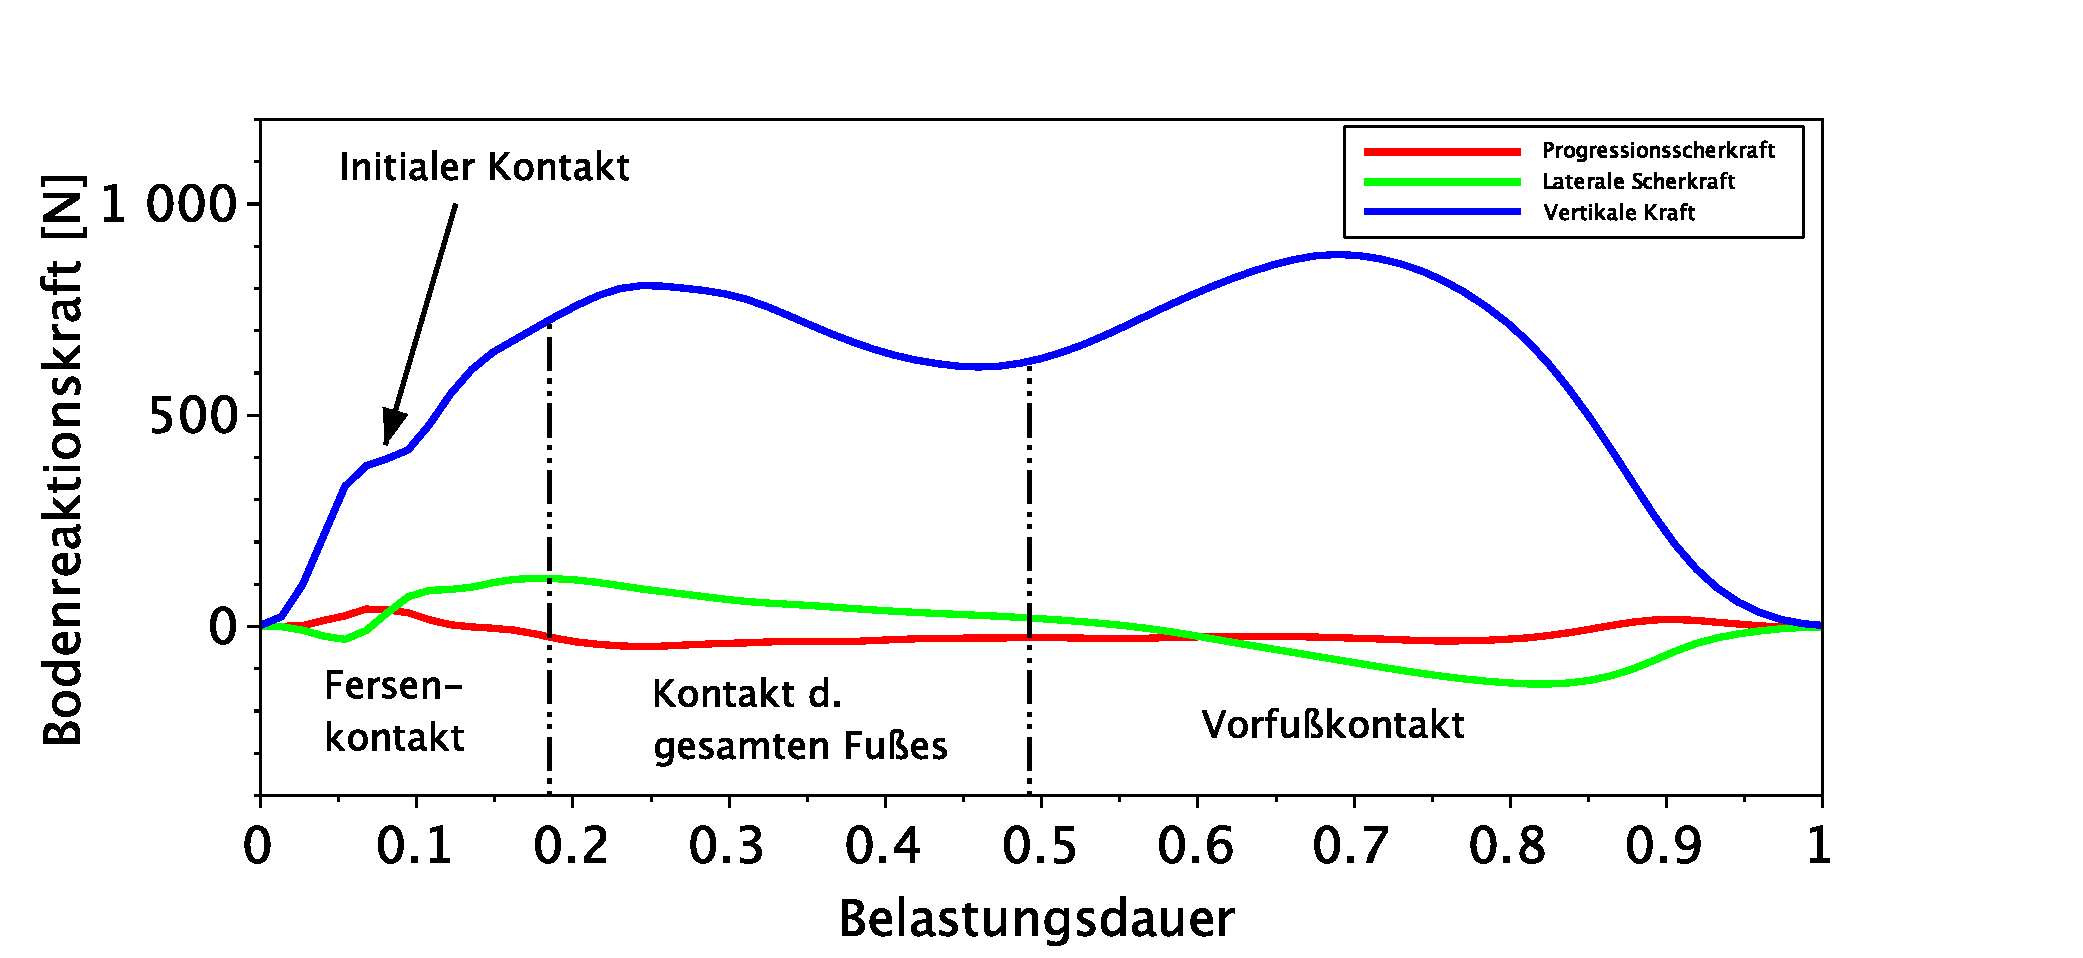
\includegraphics[width=\linewidth]{bilder/Ergebnisse/brk_annotations.pdf}
	\caption{Bodenreaktionskräfte}
	\label{fig:brk}
\end{figure}



\subsection{Vergleich Laufband}
Im Unterschied zum Laufband kommt es zu einer realen Fortbewegung im Raum, was die Frage aufwirft, ob diese beiden Bewegungsformen überhaupt vergleichbar sind. Macht es einen Unterschied, ob sich eine Person relativ zu einem bewegten Untergrund mit einer gewissen Geschwindigkeit bewegt, von einem fixen äußeren Bezugssystem (stationäre Kamera) jedoch keine Geschwindigkeit aufzuweisen scheint, oder ob sich die Person mit derselben Geschwindigkeit auf einem fixen Untergrund bewegt, betrachtet von einem bewegten Bezugssystem (bewegte Kamera).\\
Es sei vorweg genommen, dass die Beantwortung dieser Frage eine statisch relevante Methodik erfordert und die Versuchsaufbauten soweit optimiert werden müssen, dass einzig das Bezugssystem sich ändert. Dies würde bedeuten, dass die Laufstrecke so lang ist, dass keine Beschleunigungs oder Bremsvorgänge während der Aufnahme stattfinden und eine konstante, vorgegebene Geschwindigkeit eingehalten wird, wie dies auf dem Laufband der Fall ist.\\
Im Rahmen der vorliegenden Arbeit war eine solche Methodik jedoch nicht durchführbar, weshalb die folgenden Überlegungen theoretischer Natur sind, gestützt von einem Datensatz ohne Anspruch auf statistische Relevanz. 






